
\section{ТЕСТУВАННЯ ТА АНАЛІЗ РОЗРОБЛЕНОГО ПРОЄКТУ}

\subsection{Демонстрація роботи та функціональне тестування застосунку}

Для підтвердження коректності роботи розробленого програмного продукту та наочної ілюстрації його основного функціоналу покроково розглянуто основні процеси взаємодії користувача з системою. Цей процес слугуватиме для функціонального тестування ключових аспектів застосунку та підтвердження відповідності реалізованих функцій поставленим вимогам.

\subsubsection{Реєстрація та автентифікація користувача}

При першому запуску застосунку користувач потрапляє на екран автентифікації, наведений на рисунку~\ref{fig:auth}. Верхня частина екрана оформлена у вигляді брендової зони з фіолетовим градієнтним фоном та логотипом застосунку, що формує впізнаваний візуальний стиль. Нижня частина містить білу картку з двома варіантами входу до системи: формою email та пароля і кнопкою «Продовжити з Google». У правому верхньому куті розміщено перемикач мови інтерфейсу, що дозволяє обрати між українською та англійською мовами ще до входу в систему.

У разі обрання входу через Google застосунок ініціює \gls{OAuth} 2.0 потік: системний браузер відкриває сторінку авторизації Google, де користувач надає дозвіл на передачу базових даних профілю. Після успішної авторизації застосунок автоматично отримує токени доступу та зберігає сесію на пристрої, що забезпечує збереження входу між запусками без необхідності повторної автентифікації.

При вході через email та пароль облікові дані передаються на сервер через захищений канал \gls{HTTPS}. Новим користувачам доступна реєстрація за посиланням «Немає акаунту? Зареєструватись», після якої система надсилає підтвердження на email. Після успішного підтвердження та входу застосунок розпізнає активну сесію та перенаправляє користувача до головного екрана зі вкладками.

\begin{center}
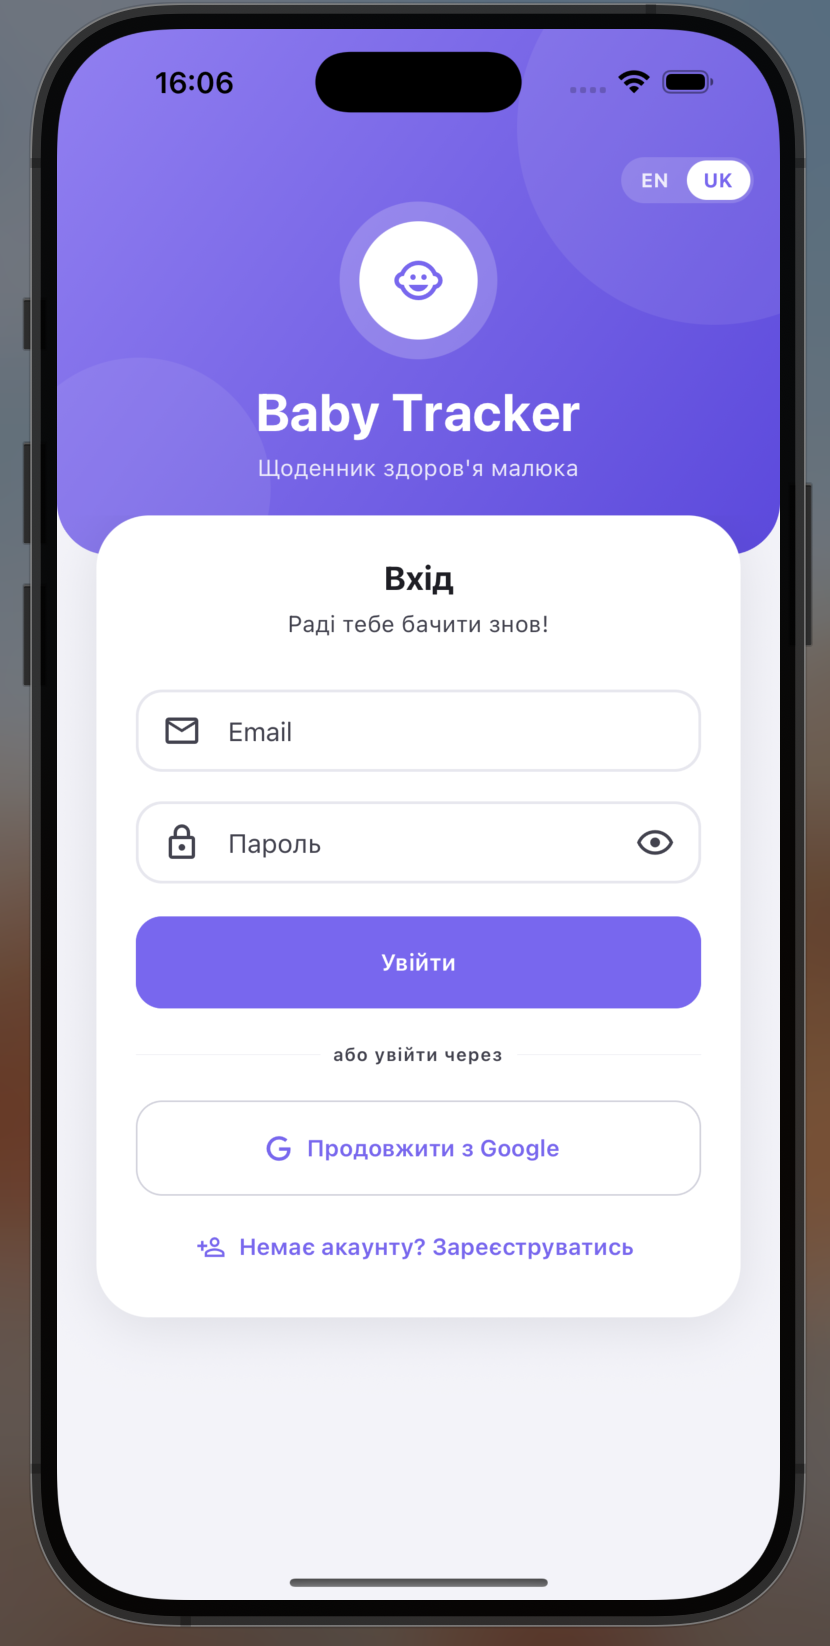
\includegraphics[height=0.5\textheight, keepaspectratio]{figures/screen-auth.png}
\captionof{figure}{Екран автентифікації застосунку}
\label{fig:auth}
\end{center}

\subsubsection{Додавання та відстеження активностей}

Після входу в систему користувач потрапляє на головний екран застосунку, наведений на рисунку~\ref{fig:home}. У верхній частині відображається вітальна картка з іменем авторизованого користувача та поточною датою. Під нею розміщено картку активної дитини з аватаром, ім'ям та кількістю повних місяців від дати народження; праворуч --- перемикач між кількома дітьми у вигляді кружальців аватарів. Нижче знаходяться три лічильники поточного дня: кількість годувань, тривалість сну та кількість змін підгузків --- вони оновлюються в реальному часі одразу після внесення кожного нового запису.

\begin{center}
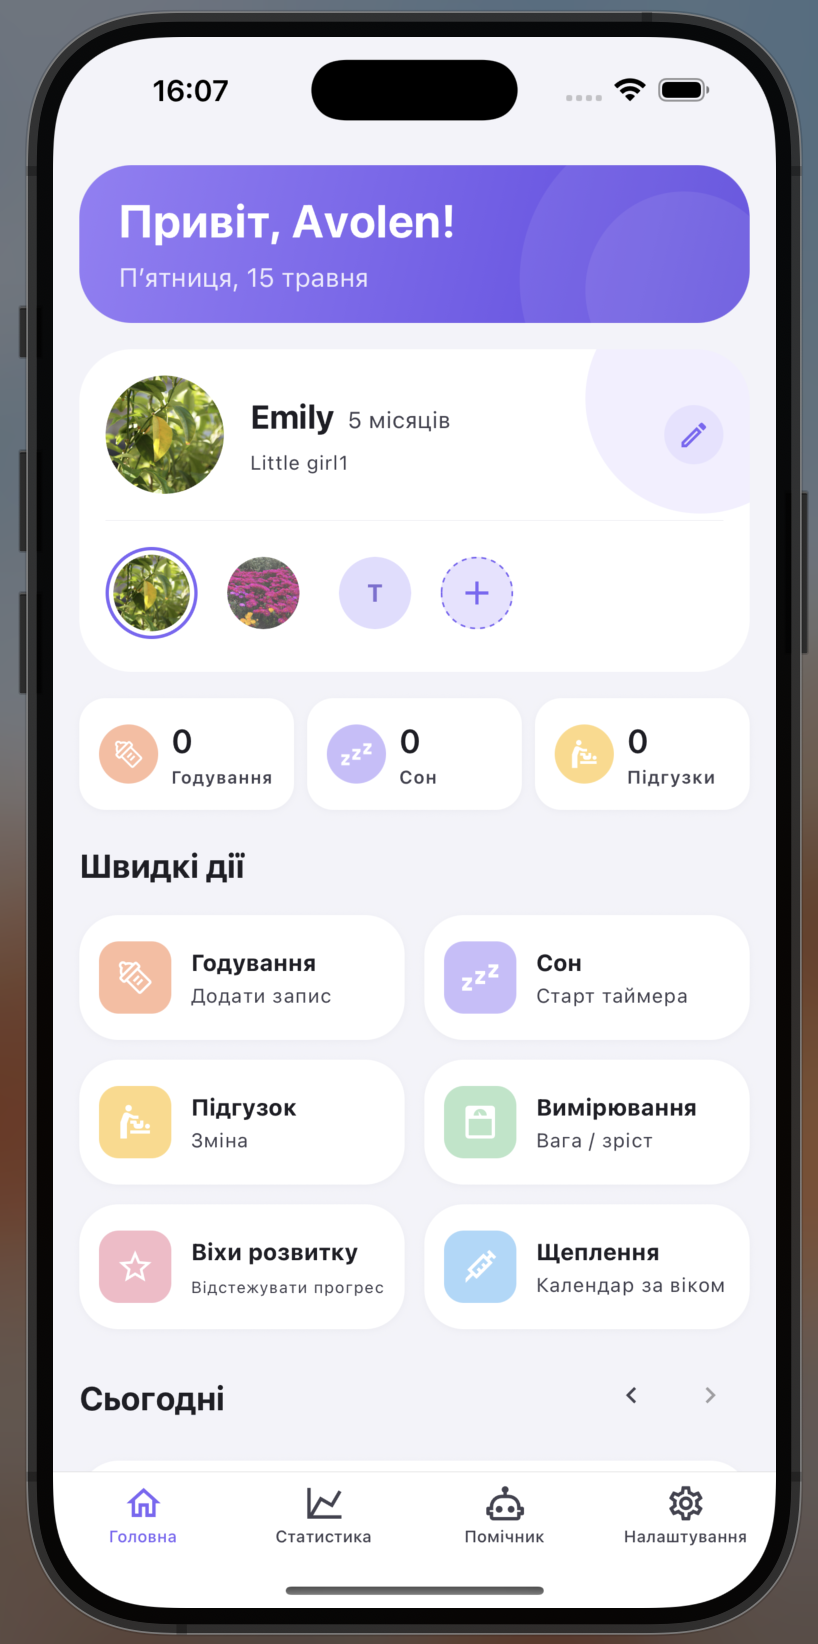
\includegraphics[height=0.5\textheight, keepaspectratio]{figures/screen-home.png}
\captionof{figure}{Головний екран застосунку}
\label{fig:home}
\end{center}

Для внесення запису годування користувач натискає картку «Годування» у сітці швидких дій. Застосунок відкриває модальну форму, наведену на рисунку~\ref{fig:feeding-form}, де у верхній частині розміщена сітка з п'ятьма типами годування: ліва груди, права груди, пляшка з грудним молоком, пляшка з сумішшю та тверда їжа. Кожен варіант представлений карткою з кольоровою іконкою та текстовим підписом; активний тип підсвічується кольоровою рамкою. Після вибору типу користувач може натиснути «Старт зараз» для запуску таймера активного сеансу або вручну ввести тривалість минулого годування у полі нижче та натиснути «Зберегти».

\begin{center}
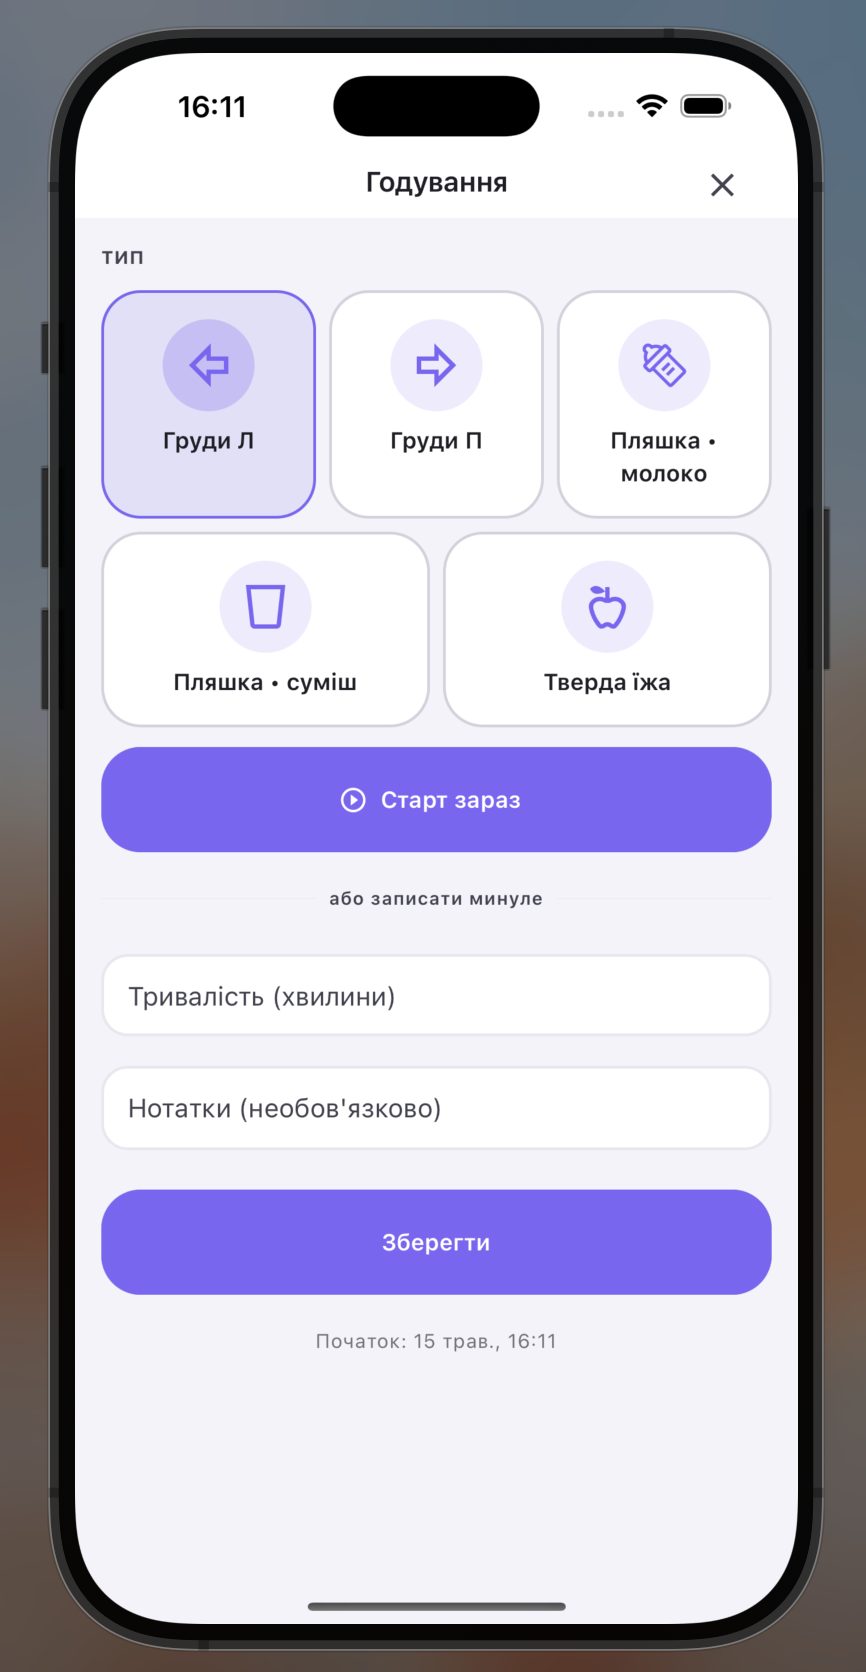
\includegraphics[height=0.5\textheight, keepaspectratio]{figures/screen-feeding-form.png}
\captionof{figure}{Форма додавання запису годування}
\label{fig:feeding-form}
\end{center}

При натисканні «Старт зараз» застосунок фіксує початок сеансу, а на головному екрані з'являється таймер з відліком тривалості поточного сеансу. При натисканні «Зупинити» сеанс завершується і новий запис одразу з'являється в хронологічній стрічці подій поточного дня у нижній частині головного екрана.

Аналогічно реалізовано журналювання сну: натискання картки «Сон» відкриває форму з вибором типу (денний або нічний) та кнопкою запуску таймера. Активний сеанс сну відображається таймером на головному екрані і завершується натисканням «Зупинити», після чого запис автоматично з'являється у стрічці поточного дня. Зміни підгузків та одиничні події --- досягнення й вакцинації --- фіксуються відповідними картками у сітці швидких дій без потреби у додаткових полях.

\subsubsection{Моніторинг антропометричних показників}

Для внесення вимірювання маси тіла, зросту або окружності голови користувач обирає картку «Вимірювання» на головному екрані. Відкривається форма з полями вибору типу показника, числового значення та одиниці вимірювання. Після збереження запис зберігається у базі даних і стає доступним у модулі статистики антропометрії. Екран вимірювань відображає окрему картку для кожного типу показника з графіком динаміки та позначенням перцентильних зон \gls{ВООЗ}.

На рисунку~\ref{fig:measurements} наведено екран антропометричного моніторингу з двома графіками: зросту та окружності голови. Для кожного показника застосунок виконує лінійну інтерполяцію між рядками перцентильних таблиць і обчислює п'ять граничних значень: P3, P15, P50, P85 та P97 для точного вікового значення дитини. Фон графіка розфарбовується відповідно до зони, в яку потрапляє значення: зелена зона між P15 та P85 відповідає нормі, жовті зони --- граничним значенням P3--P15 та P85--P97, червоні зони --- відхиленням нижче P3 та вище P97. Під кожним графіком відображається текстова класифікація останнього виміряного значення.

Під графіком кожного показника розміщена кнопка переходу до повної хронологічної історії вимірювань, наведеної на рисунку~\ref{fig:history}. Записи згруповані за датою у порядку спадання та містять тип показника, числове значення і точний час внесення. Такий підхід дозволяє батькам відстежувати довгострокову динаміку фізичного розвитку дитини і виявляти систематичні відхилення задовго до їх перетворення на клінічно значущі. У разі виявлення значень у червоній зоні (нижче P3 або вище P97) батькам рекомендується консультація педіатра для виключення патологічних причин відхилення.

\begin{center}
\begin{minipage}{0.45\textwidth}
  \centering
  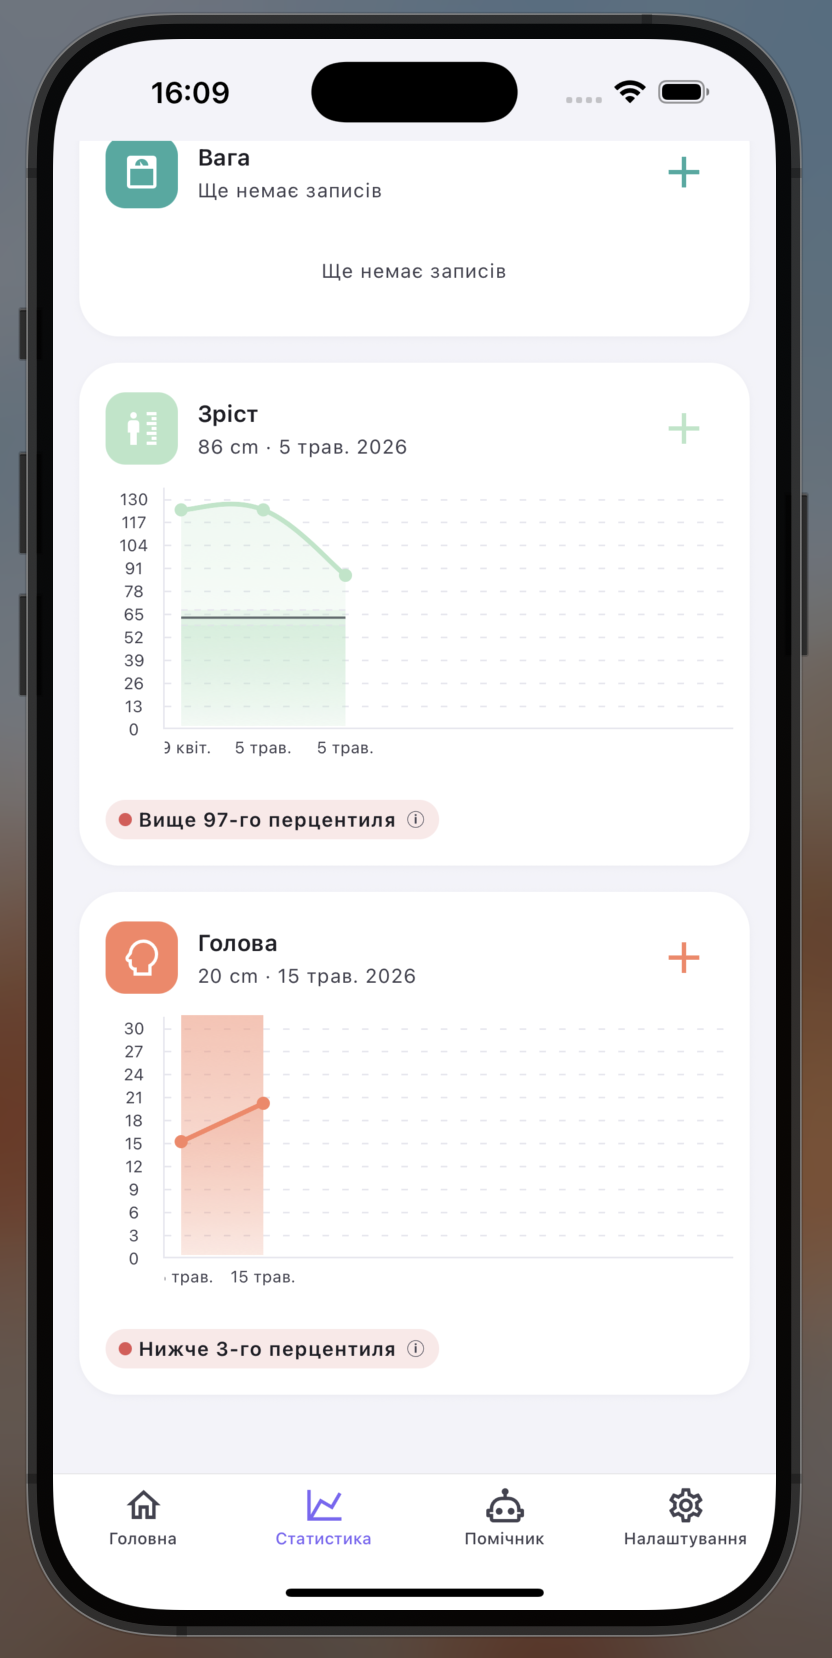
\includegraphics[height=0.45\textheight, keepaspectratio]{figures/screen-measurements.png}
  \captionof{figure}{Екран вимірювань із перцентильними зонами}
  \label{fig:measurements}
\end{minipage}
\hfill
\begin{minipage}{0.45\textwidth}
  \centering
  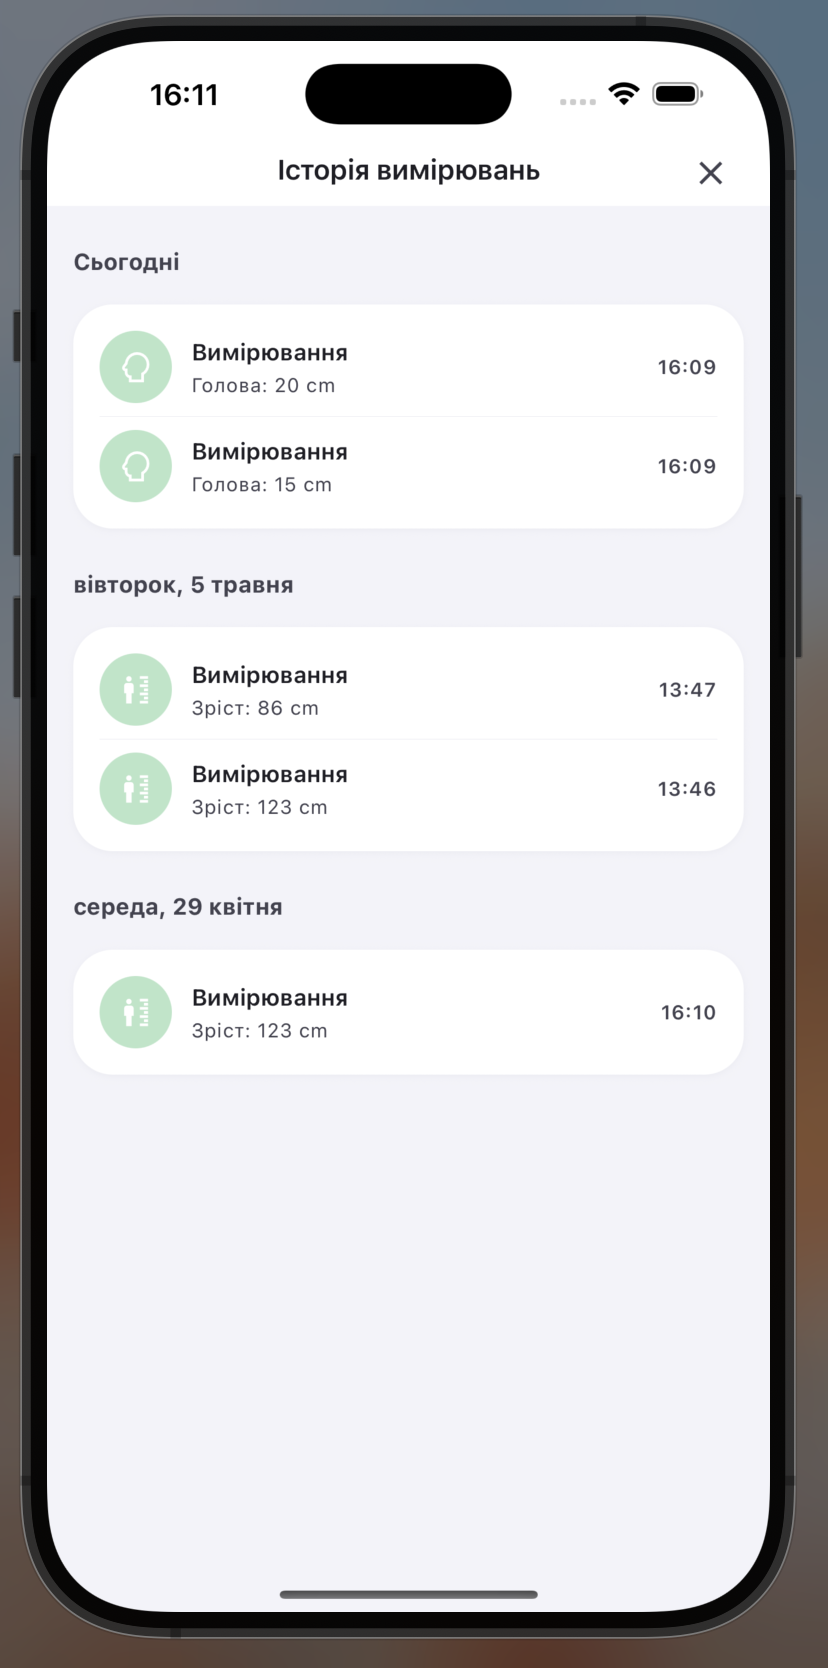
\includegraphics[height=0.45\textheight, keepaspectratio]{figures/screen-history.png}
  \captionof{figure}{Екран історії вимірювань}
  \label{fig:history}
\end{minipage}
\end{center}

\subsubsection{Аналітика активностей}

Екран статистики, наведений на рисунку~\ref{fig:stats}, відображає аналітику за останні 7 днів у вигляді трьох стовпчастих графіків: кількість годувань, загальна тривалість сну та кількість змін підгузків по днях тижня. Кожен стовпець відповідає одному дню, що дозволяє одразу побачити тенденції та відхилення від звичного режиму дитини.

Для глибшого аналізу режиму сну реалізовано окремий графік розподілу сну за часом доби: вісь Y відображає години від 00:00 до 24:00, а кожен стовпець показує діапазон активного сну у відповідний день, що дозволяє візуально виявляти порушення нічного режиму або надмірний денний сон. Під графіком сну відображається підсумковий рядок із загальною тривалістю денного та нічного сну за тиждень. Якщо середня кількість змін підгузків виходить за межі норми, екран відображає відповідне попереджувальне повідомлення.

\begin{center}
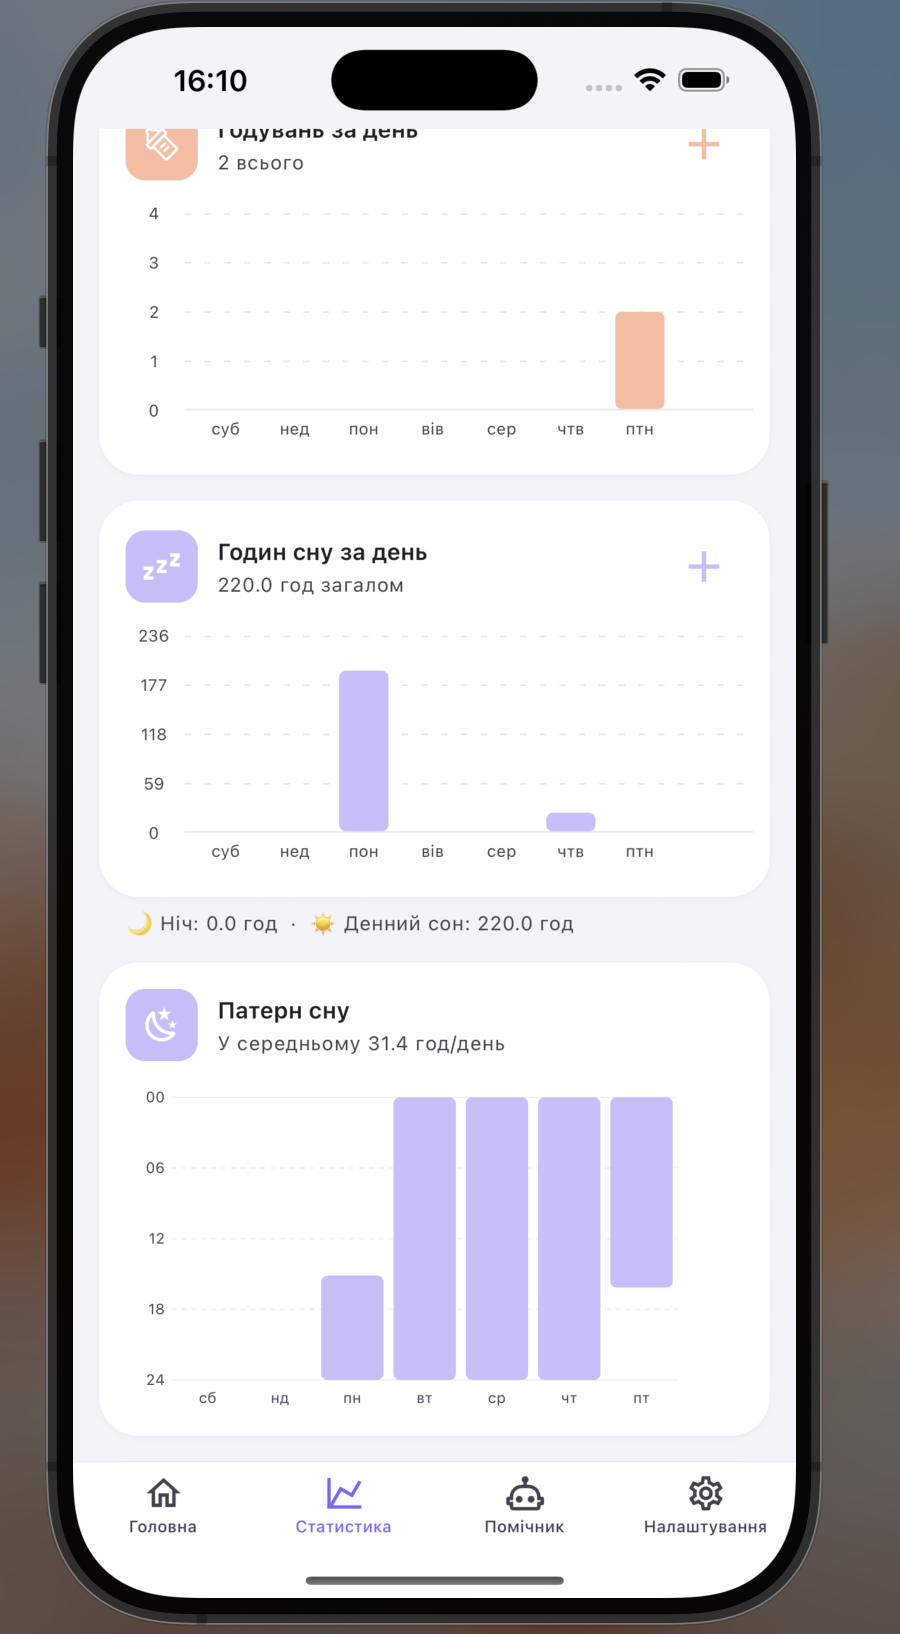
\includegraphics[height=0.5\textheight, keepaspectratio]{figures/screen-stats.png}
\captionof{figure}{Екран статистики за 7 днів}
\label{fig:stats}
\end{center}

\subsubsection{Налаштування застосунку}

Екран налаштувань, наведений на рисунку~\ref{fig:settings}, організований у три тематичні секції. Секція «Профіль» надає доступ до редагування імені та адреси електронної пошти, а також до зміни пароля через відповідні модальні форми. Секція «Налаштування» містить перемикач мови інтерфейсу між українською та англійською, а також вибір теми оформлення; зміна мови набирає чинності миттєво без перезавантаження застосунку. Секція «Акаунт» включає кнопки виходу із системи та видалення облікового запису, кожна з яких потребує підтвердження у діалоговому вікні для запобігання випадковим деструктивним діям.

\begin{center}
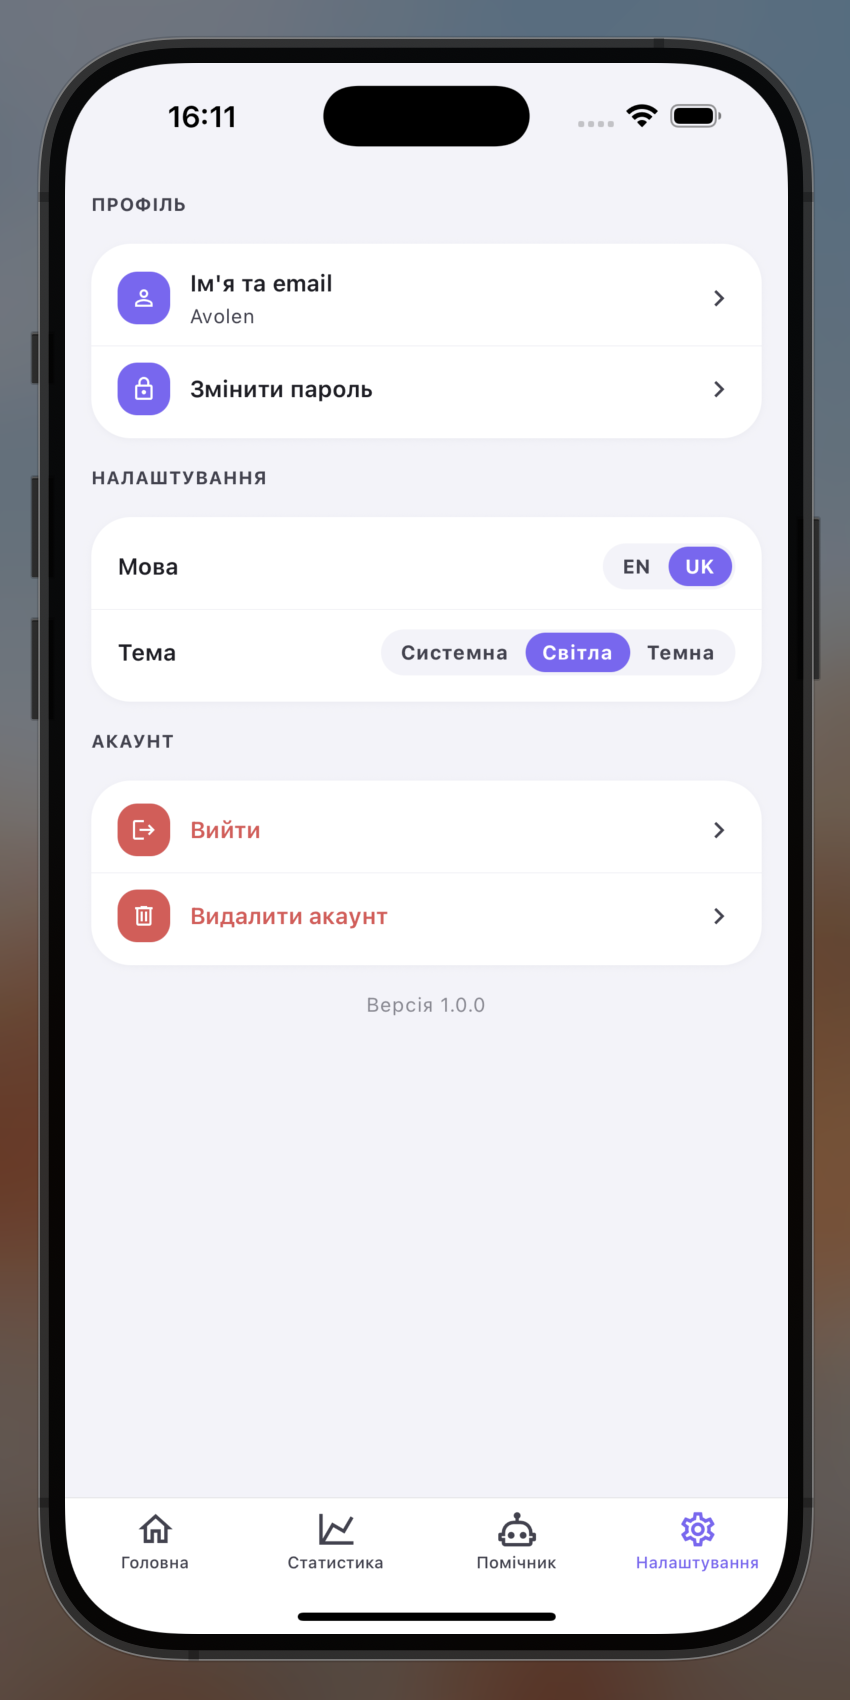
\includegraphics[height=0.5\textheight, keepaspectratio]{figures/screen-settings.png}
\captionof{figure}{Екран налаштувань застосунку}
\label{fig:settings}
\end{center}

Після покрокової демонстрації основних сценаріїв взаємодії з системою розглянемо результати тестування її ключових функціональних модулів.

\subsection{Тестування ключових функцій системи}

\subsubsection{Модульне тестування бізнес-логіки}

Для верифікації коректності бізнес-логіки, що не залежить від компонентів \gls{UI}, реалізовано набір модульних тестів з використанням фреймворку Jest у поєднанні з пресетом \texttt{jest-expo} та препроцесором \texttt{ts-jest}, що дозволяє виконувати TypeScript-тести безпосередньо в середовищі Node без попередньої компіляції. Для тестування React-компонентів інтегровано бібліотеку \texttt{@testing-library/react-native}, яка надає утиліти для рендерингу компонентів у тестовому оточенні та перевірки їх поведінки за доступністю, а не за внутрішньою структурою.

Тести організовано у директорії \texttt{app/\_\_tests\_\_/} із дзеркальною структурою відносно основного коду. Покрито шість функціональних областей:

\begin{itemize}
  \item \texttt{features/measurements/who.test.ts} --- тести алгоритму перцентильної класифікації: перевірка інтерполяції між суміжними місяцями, повернення \texttt{null} для віку понад 24 місяці, відмінність P50 між статями, коректність меж перцентильних зон;
  \item \texttt{lib/age.test.ts} --- тести функції форматування віку дитини: коректне відображення у днях, тижнях, місяцях та роках залежно від вікового діапазону, обробка майбутніх дат народження;
  \item \texttt{lib/aggregate.test.ts} --- тести агрегації активностей по днях: коректне формування 7-денних бакетів, підрахунок подій, підсумовування зважених значень;
  \item \texttt{features/milestones/labels.test.ts}, \texttt{features/vaccinations/labels.test.ts} --- тести відображення категорій досягнень та вакцинацій;
  \item \texttt{features/errors/translate.test.ts} --- тести перекладу серверних помилок у зрозумілі повідомлення для користувача.
\end{itemize}

Оскільки тести виконуються в середовищі Node, React Native-модулі, що залежають від нативного коду, замінюються мінімальними заглушками через файл \texttt{\_\_mocks\_\_/react-native.js}. Такий підхід дозволяє запускати тести без емулятора або фізичного пристрою --- виключно з командного рядка командою \texttt{jest}.

\subsubsection{Перевірка безпеки та ізоляції даних}

Коректність роботи \gls{RLS}-політик є критично важливою вимогою для застосунку, що зберігає персональні медичні дані. Тестування проводилося з двома тестовими обліковими записами: обліковий запис А з дитиною Emily та набором записів активностей, і обліковий запис Б без жодних доданих дітей. Після входу в систему від імені облікового запису Б та виконання запиту на отримання списку дітей застосунок повернув порожній список, що підтверджує коректну роботу \gls{RLS}-політики для таблиці \texttt{children}.

Наступним кроком перевірялася ізоляція записів активностей. За умов активної сесії облікового запису Б було сформовано прямий \gls{SQL}-запит до таблиці \texttt{feedings} без фільтрів через клієнт Supabase. Незважаючи на відсутність умови \texttt{WHERE child\_id = ...} у клієнтському коді, PostgREST автоматично застосував \gls{RLS}-фільтр і повернув порожній набір рядків, оскільки обліковий запис Б не має жодного запису в таблиці \texttt{caregivers}. Це підтверджує, що захист даних реалізований не на рівні клієнтського застосунку, а на рівні \gls{СУБД}, і не може бути обійдений навіть при наявності прямого доступу до \gls{API}.

Додатково перевірялася коректність роботи тригера автоматичного призначення власника. При створенні нового профілю дитини від імені облікового запису Б у таблиці \texttt{caregivers} автоматично з'явився запис з парою (\texttt{profile\_id} облікового запису Б, \texttt{child\_id} нової дитини) та роллю \texttt{owner}. Після цього запити до \texttt{feedings} та інших таблиць активностей для цієї дитини почали повертати дані, що підтверджує коректну роботу механізму автоматичного призначення прав доступу без додаткових дій з боку клієнтського коду.

\subsubsection{Тестування синхронізації між пристроями}

Синхронізація між пристроями реалізована через Supabase Realtime та є однією з ключових конкурентних переваг системи порівняно з аналогами. Для тестування цієї функціональності застосунок було одночасно відкрито на двох пристроях --- iPhone 14 Pro та iPad Air --- під одним обліковим записом із активною дитиною Emily. Обидва пристрої підписалися на канал синхронізації для активної дитини, що відстежує зміни в усіх таблицях активностей.

При додаванні нового запису про годування на першому пристрої було зафіксовано час від збереження форми до появи нового запису у стрічці подій на другому пристрої. У трьох незалежних вимірюваннях цей час склав 1,2, 1,4 та 1,8 секунди відповідно, в середньому --- близько 1,5 секунди. Такий час відгуку є цілком прийнятним для сценарію спільного ведення записів двома батьками і не потребує ручного оновлення сторінки. Аналогічний результат отримано при запуску та зупинці таймера сну: зміна стану активного сеансу миттєво відображалася на обох пристроях.

Механізм синхронізації коректно обробляв і конкурентні сценарії: при одночасному додаванні двох різних записів з обох пристроїв обидва записи з'явилися у стрічці подій на кожному пристрої без конфліктів або втрат даних. PostgreSQL забезпечив атомарність кожної вставки на рівні транзакцій, а Supabase Realtime доставив події оновлення незалежно для кожного запису. Таким чином, архітектурне рішення щодо використання Realtime-підписок у поєднанні з інвалідацією кешу TanStack Query продемонструвало надійну роботу в умовах паралельної взаємодії кількох клієнтів з одними даними.

\subsection{Аналіз результатів тестування}

Модульні тести повністю пройшли на всіх шести охоплених функціональних областях без помилок. За результатами проведеного функціонального тестування всі ключові сценарії взаємодії користувача з системою виконались коректно. Автентифікація через email та Google \gls{OAuth} функціонує стабільно на обох платформах --- iOS та Android. Журналювання всіх шести типів активностей (годування, сон, підгузок, вимірювання, досягнення, вакцинація) виконується без помилок, з правильним збереженням усіх полів у базі даних та коректним відображенням у хронологічній стрічці подій.

Алгоритм класифікації антропометричних показників за стандартами \gls{ВООЗ} продемонстрував коректну роботу на тестових наборах даних. Значення зросту 86 см для дитини у 5 місяців правильно класифікується як «Вище 97-го перцентиля», оскільки це значення суттєво перевищує верхню межу норми для цього вікового діапазону. Значення окружності голови 20 см для тієї самої дитини коректно класифікується як «Нижче 3-го перцентиля». Обидві класифікації збігаються з розрахунковими значеннями перцентильних таблиць \gls{ВООЗ}, підтверджуючи правильність реалізованого алгоритму лінійної інтерполяції.

Тестування безпеки підтвердило повну ізоляцію даних між обліковими записами на рівні \gls{СУБД}. Синхронізація між пристроями в реальному часі продемонструвала затримку близько 1,5 секунди, що є прийнятним показником для даного класу застосунків.

\subsection{Розгортання та налаштування застосунку}

Розгортання бекенду виконується через Supabase Dashboard. Спочатку створюється новий проєкт із вибором географічного регіону розміщення сервера. Після ініціалізації проєкту застосовується схема бази даних через виконання SQL-міграційних файлів у редакторі Dashboard: створюються всі десять предметних таблиць, визначаються \gls{RLS}-політики та тригер призначення власника. Паралельно в розділі Auth активується провайдер Google OAuth із введенням Client ID та Client Secret, отриманих у Google Cloud Console, а також визначаються допустимі URL-адреси перенаправлення для deep-link застосунку.

Збірка та публікація клієнтського застосунку виконується через Expo Application Services. Конфігурація проєкту описана у файлі \texttt{app.json}, де визначаються ідентифікатор пакету (\texttt{com.babyjourney.app}), версія, дозволи та конфігурація глибоких посилань для \gls{OAuth}. Змінні середовища --- URL та анонімний ключ Supabase --- зберігаються у файлі \texttt{.env} та передаються до збірки через механізм EAS Environment Variables. Команда \texttt{eas build -{}-platform ios -{}-profile production} ініціює хмарну збірку на серверах Expo; після її завершення артефакт \texttt{.ipa} готовий до відправки в App Store Connect. Аналогічна команда для платформи Android генерує \texttt{.aab}-файл для завантаження у Google Play Console.

Для автоматизації контролю якості коду налаштовано конвеєр безперервної інтеграції на базі GitHub Actions. При кожному push до гілки \texttt{main} та при створенні pull request автоматично запускається послідовність із трьох перевірок: статичний аналіз коду інструментом ESLint (\texttt{npx expo lint}), перевірка типів компілятором TypeScript у режимі \texttt{--noEmit} та виконання повного набору модульних тестів командою \texttt{npm test -{}-ci}. Конвеєр виконується на хмарному агенті Ubuntu з Node.js версії 20 і використовує кешування залежностей npm для скорочення часу виконання. Така автоматизація унеможливлює злиття коду з типовими помилками TypeScript або регресіями у тестах, забезпечуючи стабільність основної гілки репозиторію на всіх етапах розробки.

\begin{unnumbered}

\section{ВИСНОВОК ДО РОЗДІЛУ 4}

У четвертому розділі проведено демонстрацію роботи та функціональне тестування розробленої кросплатформної системи агрегації та обробки медико-біологічних даних.

Покроково розглянуто основні сценарії взаємодії користувача з системою: реєстрацію та автентифікацію через email/пароль та Google \gls{OAuth}, журналювання активностей із підтримкою активних таймерів сну та годування, а також моніторинг антропометричних показників із класифікацією за стандартами \gls{ВООЗ}. Усі розглянуті сценарії виконались коректно відповідно до очікуваної поведінки.

Верифіковано коректність бізнес-логіки за допомогою набору модульних тестів, що покривають алгоритм перцентильної класифікації, агрегацію активностей та форматування вікових показників. Підтверджено коректну ізоляцію даних між обліковими записами на рівні \gls{RLS}-політик PostgreSQL: жоден із тест-кейсів не виявив витоку даних. Тестування синхронізації між двома пристроями підтвердило стабільну роботу Supabase Realtime із середньою затримкою 1,5 секунди при паралельній взаємодії кількох клієнтів.

Описано процес розгортання бекенду на платформі Supabase та збірки клієнтського застосунку через Expo Application Services для платформ iOS та Android, що завершує повний цикл розробки програмного продукту.

\end{unnumbered}
